\lab{Application}{Depth and Breadth First Search with Kevin Bacon}{Depth and Breadth First Search with Kevin Bacon}
\label{lab:SixDegreesKevinBacon}
<<<<<<< HEAD
\objective{This section teaches about searching graphs and uses the parlor game ``Six Degrees of Kevin Bacon'' as an application to graphs.}
=======
\objective{This section teachings about searching graphs and uses the parlor game the Six Degrees of Kevin Bacon as an application to graphs}
>>>>>>> develop

\section*{Searching Graphs}
There are two common ways to search a graph;
the method used depends on the desired solution.
One method is called a depth first search (DFS).  It is designed to search the deepest levels of a graph first.
The other method is a breadth first search (BFS).  BFS searches the graph one level at a time until a solution is found.
\begin{figure}[h]
\centering
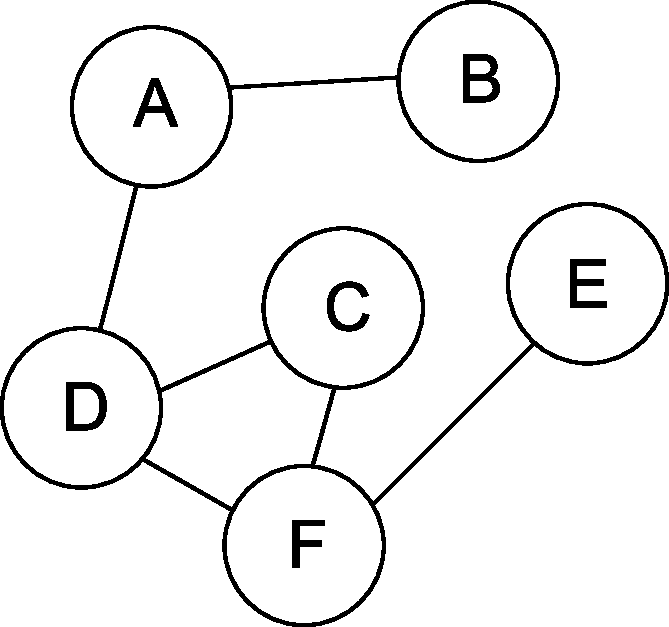
\includegraphics[width=.5\textwidth]{graph.pdf}
\caption{An example graph.}
\label{fig:bfs_dfs_graph}
\end{figure}

We call where the algorithm begins the root node.
Here, we will walk through two examples of a DFS.
In these examples, when a node has multiple branches originating from it, we visit the latest (greater) letter in the alphabet first.
First, we will use D as the root node and E will be our target node.
Starting at D, we look at its greatest neighbor, F, then F's greatest neighbor E.
Since E was our target, the algorithm ends.

Second, we will start with A and search for B.
We visit nodes A, D, F, E.
At this point, we have gone as deeply as we can go and have not found node B.
So, we back up and try another branch of nodes.
The algorithm backtracks to F and tries another route, visiting C.
Since we have marked D as already visited, we go no further.
(This is important, otherwise DFS will loop infinitely around the cycle in the graph.)
We back up again to F.  We have tried all possible branches from F, so we back up again to D.
We have exhausted all sub-branches originating from D so we travel back to A and try any unexplored branches.
We then find B and the algorithm ends.

Let's try the same two searches with BFS.
In the first search, we start at D and look for E.
We search for E among the neighbors of D: A, C, and F.
We have not found E, so we search among the the neighbors of A, C, and F (that we have not already visited).
We look at A first because A precedes C and F.
B is the only neighbor of A that we have not visited; we therefore backtrack to the neighbors of D.
We have already visited both neighbors of C, so we continue to F. Finally, we find E (the only unvisited neighbor of F) and the algorithm ends.

In the second search, we start with A.
Since B is a neighbor of A, we find it immediately.

Both DFS and BFS have advantages.
If we can choose a root node that is in some way local to the target node, BFS is obviously the better choice.
DFS, in some case, is much more efficient when the solution is far from the target node.
DFS can also be implemented very elegantly as a recursive algorithm (an algorithm that references itself to solve a smaller sub-problem).
However, with large graphs, a recursive algorithm will not perform very well computationally.

\begin{algorithm}
\begin{algorithmic}[1]
\Procedure{BFS/DFS}{$G, root, destination$}
	\State $Q \gets \text{Deque (BFS) or list (DFS) with root node in it}$	\Comment{Initialization steps}
	\State $marked \gets \text{Set with root node in it}$	
	\State $visited \gets \text{empty list}$	
	\While{$Q \text{ has elements}$}						\Comment{Go through the graph}
		\State $t \gets Q\text{'s left (BFS) or right (DFS) element}$	
		\State $\text{add }t \text{ to the visited list}$
		\If{$t==destination$}							\Comment{Found the destination node}
			\State \pseudoli{return} $t,visited$
		
		\Else										\Comment{Visit $t$'s neighbors}
			\For{$k \text{ in the adjacent nodes of } t$}
				\If{$k \text{ not in } marked$}
					\State $\text{add } k \text{ to } marked$
					\State $\text{add } k \text{ to } Q$
				\EndIf
			\EndFor
		\EndIf
	\EndWhile
\EndProcedure
\end{algorithmic}
\caption{Breadth first and depth first search}
\label{alg:BFSDFS}
\end{algorithm}

\begin{problem}
Implement methods that will perform depth first and breadth first searches on a graph.
Use a \li{set()} to store the visited nodes.
A set data structure supports very efficient membership testing because
sets are often implemented using binary search trees.

\textit{Hint: The implementations of depth first and breadth first search are exactly same with one very important difference.
The difference is how a particular data structure is used.  What data structure is used differently and how is it used differently?}
\end{problem}

\section*{Shortest Path Algorithms for Unweighted Graph}
Let $A$ be a unweighted graph. How can we find the shortest path between two nodes?  One way is by doing a breadth first search and stopping when we reach the target node. The downside to doing it this way is that the algorithm will look through every node on every level before it reaches the target node. Let us pretend that for two nodes $a, b \in A$ that the distance between $a$ and $b$ is 5. Also suppose that, in going from $a$ to $b$, you have to check $2^n$ elements where $n$ in the level. So 2 nodes are one away from $a$, 4 nodes are two away from $a$, and so on. Then you would have to check at least 32 nodes before you would get to $b$.

A better way to find the shortest path is to do a breath first search from both $a$ and $b$. So you calculate all the nodes one away from $a$ and all the nodes one away from $b$, then two away from $a$ and two away from $b$, and so on until you find a node that is connected to both $a$ and $b$. Using the same example as before, if you assume there is $2^n$ nodes at the nth level away from $b$ then the number of nodes you have to check before reaching the shortest path is at least 12 and at most 20.

When you have many more nodes each level away, the speedup from doing a breath first search from both sides is much greater. This is one of the best ways to find shortest paths in unweighted, undirected graphs. For weighted graphs there are many algorithms that find the shortest path. For further information look at Dijkstra's algorithm, Bellman–Ford algorithm, A* search algorithm, Floyd–Warshall, and Johnson's algorithm.

\section*{Six Degrees of Kevin Bacon}
\begin{figure}[h]
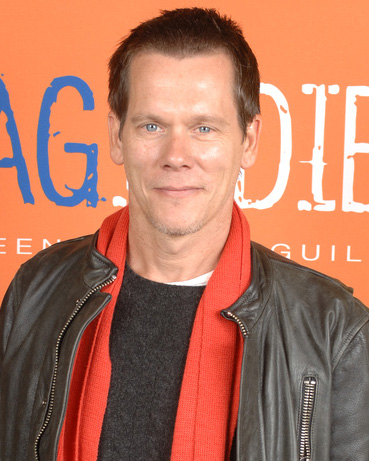
\includegraphics[scale = .4]{Kevin_Bacon.jpg}
\caption{Kevin Bacon.  Image source: Wikipedia.}
\end{figure}

Kevin Bacon is a famous actor who has been in a lot of movies. The six degrees of Kevin Bacon came from a comment made in an interview where Bacon said that he had worked with everyone in Hollywood or someone who's worked with them.  The idea is that you can connect actors to Kevin Bacon. Each actor has a Bacon number that is found as follows:
\begin{enumerate}
\item Kevin Bacon has a Bacon number of 0.
\item Actors that have been in a movie with Kevin Bacon have a Bacon number of 1.
\item For all other actors $X$, if the lowest number of any actor that $X$ has been in a film with is $n$, $X$ has a Bacon number of $n+1$.
\end{enumerate}

\begin{figure}[h]

\includegraphics[scale = .6]{Example}
\caption{Jeffery Humphery was in \emph{End Game} with Cuba Gooding Jr. who was in \emph{A Few Good Men} with Kevin Bacon, so Jeffrey Humphrey has a Bacon Number of 2.  Image source: http://oracleofbacon.org/.}
\end{figure}

You can define a graph in the same way: where each actor is a node and there is an edge between any two nodes if the actors were in a movie together. From this you can find the shortest path between any actor and Kevin Bacon by using any of the algorithms listed above. Of course, this can be done with any actor and just not Kevin Bacon. There are equivalents in other fields, the most famous being the Erdos numbers: how far away you are to publishing a paper with the prolific mathematician Paul Erdos.

\section*{NetworkX}
For this lab, we are going to use a network library called NetworkX. NetworkX allows us to create and manipulate large, complex networks.  Since NetworkX uses Python objects to represent its graphs internally, graphs with lots of nodes will take a large chunk of memory.  Other network libraries exist which are written in C++, like igraph, which may significantly reduce the overhead of storing the graph.
To make an undirected graph in NetworkX you do the following:
\begin{lstlisting}
import networkx as nx
G = nx.Graph()
\end{lstlisting}
To add nodes you use the \li{add_node(x)} method where $x$ is the node you want to add.  If you add an edge between two non-existent nodes, the missing nodes will also be added to the graph. Adding an edge is done by the \li{add_edge(x,y)} method where $x$ and $y$ are previously added nodes. You can add multiple edges or nodes with the \li{add_edges_from()} and \li{add_nodes_from()} methods respectively.  There are also \li{has_node(x)} and \li{has_edge(x,y)} that tell you if the node or edge is already added.
\begin{lstlisting}
G.add_node(x)
G.add_edge(x, y)
\end{lstlisting}

\begin{problem}
The data file, \texttt{movieData.txt}, contains the entire casts of movies made from 2011 to August of 2013. The file is a delimited file with each field delimited by the '/' character.
Write a method that will open the file, generate a NetworkX graph, and return the constructed graph.
For later solutions, it might be beneficial to also construct a lookup table that maps actors to the movies that they appeared in.
\end{problem}

The \li{shortest_path(G, x, y)} function in NetworkX outputs a list that is one of the shortest paths between $x$ and $y$ in graph $G$.  In an unweighted graph, it finds the shortest path using a pair of breadth first searches originating at the two target nodes.  It advances each breadth first search until they meet and then  constructs the shortest path of nodes between them.  If no target is specified, the function will find the shortest paths between $x$ and every other node in the network.  It will return the results in a dictionary.  If more than one ``shortest path'' exists, it will return the first one it finds.  We can find the length of the shortest path using the \li{shortest_path_length(G, x, y)} function.

\begin{problem}
Find the shortest path between Kevin Bacon and Liam Neeson. Then find the shortest path from Kevin Bacon to Imran Zahid. Write a function that will accept a path and output the path with the movies in between that connect the actors. Output the paths from Kevin Bacon to Liam Neeson and Imran Zahid with the connecting movies.
\end{problem}

\begin{problem}
Find the average Bacon number for the dataset. Then find how many people have each Bacon number and how many people are not connected to Kevin Bacon at all(these people have a Bacon number of infinity).
\end{problem}

